\documentclass[a4paper]{article}
\usepackage{a4wide}
\usepackage{graphicx}
\usepackage[T1]{fontenc}
\usepackage[utf8]{inputenc}
\usepackage[UKenglish]{babel}
\usepackage{placeins}
\usepackage{siunitx}
\sisetup{locale = UK}
\usepackage{color}
\usepackage{amsmath}
\usepackage{amssymb}
\usepackage{mathtools}
\usepackage{dsfont}
\usepackage{slashed}
\usepackage[backend=bibtex,style=ieee,citestyle=numeric-comp]{biblatex}
\addbibresource{bibliography.bib}
\usepackage{hyperref}

\graphicspath{{figures/}}
\newcommand{\inputtwofigs}[2]{\resizebox{0.443\textwidth}{!}{{\Large\input{#1}\input{#2}}}}

\DeclareMathOperator{\im}{i}
\DeclareMathOperator{\real}{Re}
\DeclareMathOperator{\res}{Res}
\DeclareMathOperator{\tr}{Tr}
\DeclareMathOperator{\asinh}{asinh}
\DeclareMathOperator{\acosh}{acosh}
\DeclareMathOperator{\ord}{\mathcal{O}}
\newcommand{\matr}[2]{\left(\begin{array}{#1}#2\end{array}\right)}
\newcommand{\del}[2]{\ensuremath{\frac{\partial #1}{\partial#2}}}
\newcommand{\eto}[1]{\ensuremath{\mathrm{e}^{#1}}}
\newcommand{\md}{\ensuremath{\mathrm{d}}}
\newcommand{\mD}{\ensuremath{\mathcal{D}}}
\newcommand{\ordnung}[1]{\ensuremath{\ord\left(#1\right)}}
\newcommand{\erwartung}[1]{\ensuremath{\left\langle#1\right\rangle}}

\newcommand{\kappadelta}{\ensuremath{\tilde{\kappa}}}

\newcommand{\todo}[1]{\textbf{\color{red}TODO: #1}}

\newcommand{\bonn}{
	\\\textit{\footnotesize Helmholtz-Institut f\"{u}r Strahlen- und Kernphysik,
	Rheinische Friedrich-Wilhelms-Universit\"{a}t Bonn, Germany}
}

\newcommand{\liverpool}{
\\\textit{\footnotesize Department of Mathematical Sciences,
	University of Liverpool, United Kingdom}
}

\pagestyle{headings}

\begin{document}
	\title{The Free Fermion Correlator}
	
	\author{Johann Ostmeyer\liverpool}
	\date{\today}
	\maketitle
	
	\begin{abstract}
		Some analytic and perturbative investigations of the domain wall free fermion correlator functions.
	\end{abstract}

	\allowdisplaybreaks[1]

	\section{Exact formula of the zero-momentum correlator}
	Our starting point are the formulae (20-23) combined with (38) in Ref.~\cite{hands_thirring2016} where the free fermion propagator is derived in momentum space. Very long and tedious but in principle straight forward calculations\footnote{Mostly the calculations have been performed by Mathematica, though some human interference in crucial moments proved necessary.} yield the explicit form
	\begin{align}
		C_h(p=(p_0,0,0)) &= \frac{2 \im m \sin (p_0)+2 \cos (p_0)+\sqrt{5-4 \cos (p_0)}-1}{\im \left(m^2+1\right) \sin (p_0)+2 m \cos (p_0)-m}\label{eq:exact_mom_prop_h}
	\end{align}
	in the large $L_s$ limit and setting the domain wall height $M=1$ immediately. We note at this point that perturbative expansions in $\eto{-L_s}$ yield nonvanishing contributions of first order in both cases, $m_h$ and $m_3$, and numerically these contributions are found similar. Furthermore they become irrelevant for lattice sizes as small as $L_s=10$ justifying to conduct all successive studies in the aforementioned $L_s\rightarrow\infty$ limit.
	
	Using $m_3$ instead of $m_h$, we obtain the same expression in the $L_s\rightarrow\infty$ limit as is to be expected. The convergence turns out to be significantly faster, however, as we will discuss later on.
	%the rather cumbersome expression
	%{\fontsize{2}{2}
	%\begin{multline}
	%	C_3(p=(p_0,0,0)) = \\
	%	\frac{2 \left(-3 \sqrt{5-4 \cos (p_0)}+2 \cos (p_0) \left(\sqrt{5-4 \cos (p_0)}+2\right)-5\right) \left(-(2-4 \im) m \cos (p_0)-\im m \cos (2 p_0)+m \left(\sqrt{5-4 \cos (p_0)}+(3-3 \im)\right)+\im \sin (2 p_0)-\im \sin (p_0) \left(\sqrt{5-4 \cos (p_0)}+3\right)\right)}{\sqrt{5-4 \cos (p_0)} \left(-2 \cos (p_0)+\sqrt{5-4 \cos (p_0)}+3\right) \left(m^2 \left(-\sqrt{5-4 \cos (p_0)}\right)+\left(m^2-1\right) \cos (2 p_0)+2 \cos (p_0) \left(-m^2+\sqrt{5-4 \cos (p_0)}+3\right)-2 \sqrt{5-4 \cos (p_0)}-5\right)}\label{eq:exact_mom_prop_3}
	%\end{multline}}
	%which, to the best of our knowledge, cannot be simplified any further. Since we find excellent numerical agreement between the $m_h$ and $m_3$ cases, we are not going to pursue analytic calculations using this exact form of the latter correlator.
	
	\subsection{The free propagator in momentum space}
	Often the amount of insight and physical intuition obtained from exact analytic calculations is very limited. We are therefore going to investigate an approximation in the following that captures all the important physics without `having too many trees to see the forest'.
	
	We start out with the well known free particle propagator in continuous space\footnote{This works straight forward at zero momentum as then $p\equiv p_0$ is scalar which is the relevant case for now. But it can also be extended canonically to vectorial version.}
	\begin{align}
		C(p) &= \frac{1}{m+\im p}\,.
	\end{align}
	Going to a lattice, we have to substitute the momentum $p$ for the lattice momentum $\sin p$ (where we absorb the lattice spacing into the definition of $p$). The simplest realisation of a propagator with the correct continuum limit is then
	\begin{align}
		C(p) &= \frac{1}{m+\im \sin p}\,,
	\end{align}
	which, of course, leads to the infamous fermion doubler problem since the $\sin$-function has zeros not only at integer multiples of $2\pi$, but also at multiples of $\pi$. The domain wall approach essentially gets rid of this problem by lifting the unphysical pole near $p=\pi$ (assuming $m\ll 1$). The exact formula~\eqref{eq:exact_mom_prop_h} is a particular realisation of this requirement, and so is
	\begin{align}
		C_0(p) &= \frac{1+n(m)\cos p}{m+\im \sin p}\,,\quad n(m) \coloneqq \frac{1}{\sqrt{1+m^2}}\,.
	\end{align}

	Figure~\ref{fig:free_prop_mom_space} shows that the three propagators are quite compatible, so we are going to use the simplistic version $C_0(p)$ for further analysis.

	\begin{figure}[htp]
		\centering
		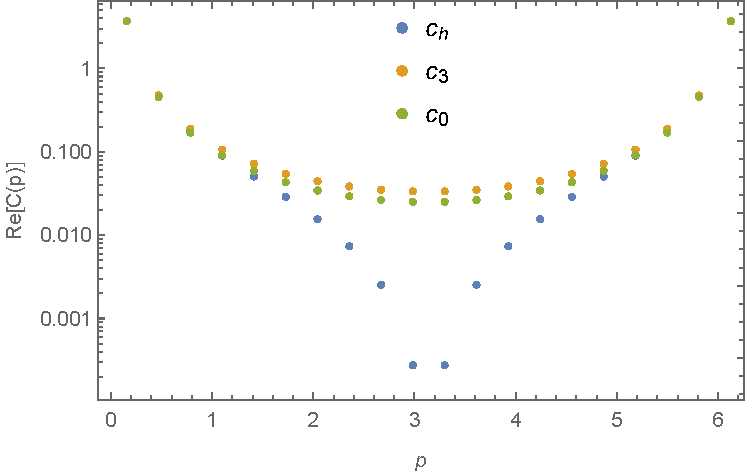
\includegraphics[width=.45\textwidth]{free-prop_mom-space}
		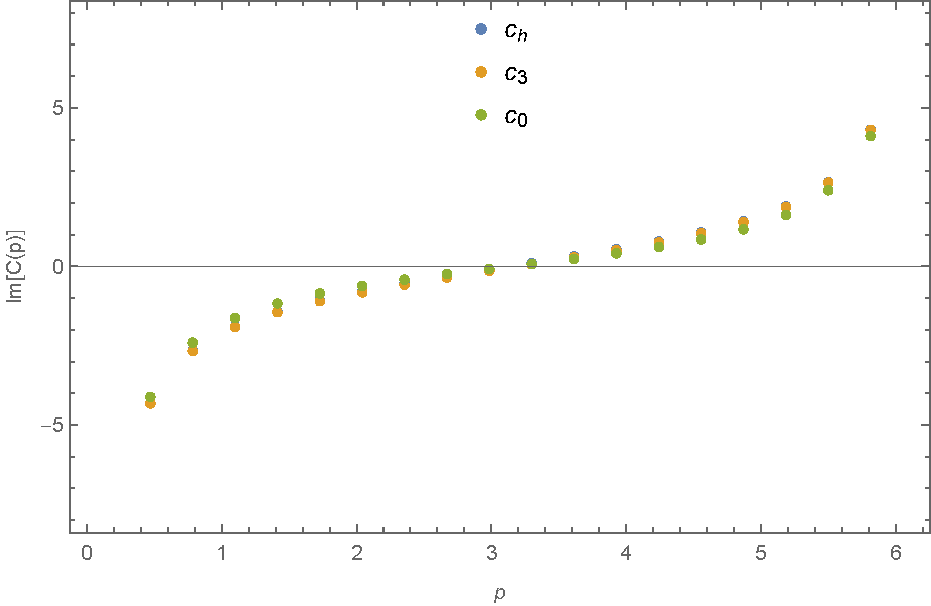
\includegraphics[width=.45\textwidth]{free-prop_mom-space_im}
		\caption{Exact and approximate free fermion propagators at zero spatial momentum in momentum space, $m=\num{0.05}$. $C_h$ and $C_3$ are identical in the visualised $L_s\rightarrow\infty$ limit. Real part left, imaginary part right.}\label{fig:free_prop_mom_space}
	\end{figure}

	\subsection{Transformation to real space}
	We are interested in the propagator in (imaginary) time, still at zero spatial momentum, so we have to perform a fermionic Fourier transformation
	\begin{align}
	C_0(t)&=\frac{1}{L_t}\sum_{p_0}C_0(p)\eto{\im p_0 t}\,.
	\end{align}
	We employ the Matsubara technique
	\begin{align}
	C_0(t)&=\frac{1}{L_t}\sum_{p_0}\frac{1+n(m)\cos p_0}{m+\im \sin p_0}\eto{\im p_0 t}\\
	&=\frac{-1}{2\pi\im}\oint_\mathcal{C}\md z\, \frac{1}{\eto{L_t z}+1}\frac{1+n(m)\cos(-\im z)}{m+\im \sin (-iz)}\eto{z t}\\
	&=\frac{-1}{2\pi\im}\oint_\mathcal{C}\md z\, \frac{\eto{z t}}{\eto{L_t z}+1}\frac{1+n(m)\cosh z}{m+\sinh z}\label{eq:contour_int_C}
	\end{align}
	where the closed contour $\mathcal{C}$ has to be chosen such that it encloses the poles of the Fermi function $\frac{1}{\eto{L_t z}+1}$ corresponding to the Matsubara frequencies $z=\im p_0=\im\frac{2\pi}{L_t}\left(j+\frac 12\right)$ with $j=0,\dots,L_t-1$ and no other poles.
	
	The integrand is $2\pi \im$-periodic (reflecting the finite momenta range due to the lattice discretisation) and has singularities at $z=\im\frac{2\pi}{N_t}\left(\mathbb Z+\frac 12\right)$, $z=-\asinh m + \im 2\pi \mathbb Z$, and at $z=\asinh m + \im \pi + \im 2\pi \mathbb Z$. The two former are poles of first order whereas the latter can be lifted, i.e.\@ the numerator is zero as well, which corresponds to the disappearance of the doubler or back-propagating part (opposite real mass) and is exactly the reason we had to introduce the normalisation $n(m)$. Thus we can safely deform the contour $\mathcal{C}$ to the four paths
	\begin{align}
	\mathcal{C}_1&=\mathbb{R}+\im \varepsilon\,,\\
	\mathcal{C}_2&=\left[\infty+\im\varepsilon,\,\infty+2\pi\im-\im\varepsilon\right]\,,\\
	\mathcal{C}_3&=-\mathbb{R}+2\pi\im-\im \varepsilon\,,\\
	\mathcal{C}_4&=\left[-\infty+2\pi\im-\im\varepsilon,\,-\infty+\im\varepsilon\right]\,.
	\end{align}
	This means that we first integrate along the real axis shifted upwards by the infinitesimal imaginary parameter $\im\varepsilon$. Then at positive real infinity we go upwards to imaginary $2\pi\im-\im\varepsilon$. Next we go in negative direction parallel to the real axis. Finally we close the contour at negative real infinity going back down to the imaginary part $\im\varepsilon$.
	
	Let us consider $\mathcal{C}_2$ and $\mathcal{C}_4$ first. $t=0,\dots,L_t-1$, therefore at positive real infinity the integrand is exponentially suppressed by the Fermi function, so $\mathcal{C}_2$ does not give any contribution. The integral along $\mathcal{C}_4$, in contrast, does not vanish for $t=0$. At negative real infinity the $\sinh$- and $\cosh$-terms dominate and the Fermi function goes to one. So we get
	\begin{align}
	\frac{-1}{2\pi\im}\int_{\mathcal{C}_4}\md z\, \frac{\eto{z t}}{\eto{L_t z}+1}\frac{1+n(m)\cosh z}{m+\sinh z}
	&=\frac{-1}{2\pi\im}\int\limits_{-\infty+2\pi\im-\im\varepsilon}^{-\infty+\im\varepsilon}\md x\, \frac{\eto{t x}}{\eto{L_t x}+1}\frac{1+n(m)\cosh x}{m+\sinh x}\\
	&=\frac{-1}{2\pi\im}\int\limits_{2\pi\im-\im\varepsilon}^{\im\varepsilon}\md x \left(-\delta_{t0}\right)\\
	&=\frac{\delta_{t0}}{2\pi\im}\left(\im\varepsilon-\left(2\pi\im-\im\varepsilon\right)\right)\\
	&=-\delta_{t0}
	\end{align}
	for $\varepsilon\rightarrow 0$.
	
	$\eto{N_t z}$ and $\sinh^2\frac z2$ are both $2\pi\im$-periodic. Thus integrating along $\mathcal{C}_3$ is identical to integrating along the real axis shifted by $-\im\varepsilon$. The union $\mathcal{C}_1 \cup \mathcal{C}_3-2\pi\im$ together with infinitesimal closing sequences at $\pm\infty$ is again a closed contour $\mathcal{C'}$ around the real axis winding once in negative direction. The corresponding integral can be performed using the residuum theorem and plugging in the single real first order pole $z_0=-\asinh m$. We get
	\begin{align}
	\frac{-1}{2\pi\im}\oint_{\mathcal{C'}}\md z\, \frac{\eto{z t}}{\eto{L_t z}+1}\frac{1+n(m)\cosh z}{m+\sinh z}
	&=\res_{z_0}\frac{\eto{z t}}{\eto{L_t z}+1}\frac{1+n(m)\cosh z}{m+\sinh z}\\
	&=\lim_{z\rightarrow z_0}\frac{\eto{z t}}{\eto{L_t z}+1}\left(1+n(m)\cosh z\right)\frac{z-z_0}{m+\sinh z}\\
	&= \frac{\eto{-\asinh m t}}{\eto{-\asinh m L_t}+1}\left(1+n(m)\cosh\asinh m\right)\frac{1}{\cosh\asinh m}\\
	&= \frac{\eto{-\tilde m t}}{\eto{-\tilde m L_t}+1}\frac{2}{\sqrt{1+m^2}}\,,
	\end{align}
	where $\tilde m\coloneqq \asinh m$.
	
	Now we have all the ingredients to evaluate equation~\eqref{eq:contour_int_C}. It yields
	\begin{align}
		C_0(t) &=
	\frac{-1}{2\pi\im}\oint_\mathcal{C}\md z\, \frac{\eto{z t}}{\eto{L_t z}+1}\frac{1+n(m)\cosh z}{m+\sinh z}\\
	&=\frac{-1}{2\pi\im}\left(\int_{\mathcal{C}_4}\md z+\oint_\mathcal{C'}\md z\right) \frac{\eto{z t}}{\eto{L_t z}+1}\frac{1+n(m)\cosh z}{m+\sinh z}\\
	&=\frac{\eto{-\tilde m t}}{\eto{-\tilde m L_t}+1}\frac{2}{\sqrt{1+m^2}}-\delta_{t0}\,,
	\end{align}
	which can easily be confirmed numerically. In the thermodynamic ($L_t\rightarrow\infty$) and continuum ($m\rightarrow0$, but $mt=\text{const.}$) limits the function approaches the expected form $\eto{-m t}$.

	\subsection{Leading order corrections}
	The propagator we derived in the previous section captures the important intermediate time $1\ll t \ll L_t$ features including some lattice artefacts and the absence of the doubler. There are, however, more subtle but still substantial discretisation effects we did not consider yet. When considering the exact form $C_h(p)$ instead of the simplified $C_0(p)$, the most prominent difference is that $C_h(p)$ has not only poles but also branch cuts due to the $\sqrt{5-4\cos p}$ - term. The square-root terms stem from the quadratic nature of $DD^\dagger$ solved for the Greens function~\cite{hands_thirring2016}, or more generally from the quadratic (chirality breaking) term of order $\ordnung{a}$ in the Ginsparg-Wilson equation~\cite{Ginsparg_Wilson}. While all the other differences are analytic and can therefore feature only in higher orders of $m$, this non-holomorphicity has an immediate impact on the contour integral and therefore on $C_h(t)$. The existence of branch cuts in the DW fermion representation has been noted before~\cite{Gavai_2009}, but to the best of our knowledge neither their origins nor their implications have been investigated so far.
	
	Branch cuts indicate unbound many-particle interactions~\cite{Peskin:1995ev}, in this case between the fermion and its doubler. These interactions are very short ranged for heavy doublers and decouple completely in the continuum limit. Put differently, the branch cuts can only start at energies larger than the sum of fermion and doubler masses and therefore vanish in the limit of infinitely heavy doublers. Here we see again that DW (or more generally Ginsparg-Wilson) fermions do not get rid of the doublers in principle, they only give zero weight to the single particle doubler poles.
	
	By and large, the derivation of $C_h(t)$ proceeds in the same way as that of $C_0(t)$ until the integral over $\mathcal C'$ has to be solved. This part turns out to be trickier as the paths $\mathcal C_1$ and $\mathcal C_3-2\pi\im$ cannot be connected at $\pm\infty$ because of the aforementioned branch cuts on the real axis starting at $\pm\acosh\frac54=\pm\ln2$. Instead we have to split both paths into three parts each
	\begin{align}
		\mathcal C_{1,3}^- &= \left[-\infty\pm\im\varepsilon,\,-\ln2\pm\im\varepsilon\right]\,,\\
		\mathcal C_{1,3}^0 &= \left[-\ln2\pm\im\varepsilon,\,\ln2\pm\im\varepsilon\right]\,,\\
		\mathcal C_{1,3}^+ &= \left[\ln2\pm\im\varepsilon,\,\infty\pm\im\varepsilon\right]
	\end{align}
	and bridge the gaps between them with infinitesimal paths orthogonal to the real axis. Thus we are left with $\mathcal C_1^0\cup\mathcal C_3^0$ enclosing the pole at $z=-\asinh m$ and yielding the same contribution as the integral over $\mathcal C'$, as well as the two paths along the branch cuts \begin{align}
		\mathcal C_\text{bc}^\pm &\coloneqq \mathcal C_1^\pm\cup\mathcal C_3^\pm\,.
	\end{align}

	Taking into account the integration directions dictated by the paths, we obtain
	\begin{align}
		\frac{-1}{2\pi\im}\int_{\mathcal{C}_\text{bc}^\pm}\md z\, \frac{\eto{z t}}{\eto{L_t z}+1}C_h(-\im z)
		&= \frac1\pi\,\Im\int_{\pm\ln2}^{\pm\infty}\md x\, \frac{\eto{t x}}{\eto{L_t x}+1}C_h(-\im x)\\
		&= \pm\frac1\pi\,\Im\int_{\ln2}^{\infty}\md x\, \frac{\eto{\pm t x}}{\eto{\pm L_t x}+1}C_h(\mp\im x)\\
		&\approx \pm\frac1\pi\,\Im\int_{\ln2}^{\infty}\md x\, \frac{\eto{\pm t x}}{\eto{\pm L_t x}+1}\frac{\sqrt{5-4 \cosh x}}{m\pm\sinh x}\\
		&= \pm\frac1\pi\int_{\ln2}^{\infty}\md x\, \frac{\eto{\pm t x}}{\eto{\pm L_t x}+1}\frac{\sqrt{4 \cosh x-5}}{m\pm\sinh x}\,.
	\end{align}
	To the best of our knowledge this integral has no exact analytic solution, so we used an approximation again, this time taking the scaling near $\ln2$ and the asymptotic behaviour into account:
	\begin{align}
		\frac{-1}{2\pi\im}\int_{\mathcal{C}_\text{bc}^+}\md z\, \frac{\eto{z t}}{\eto{L_t z}+1}C_h(-\im z)
		&\approx \frac1\pi\int_{0}^{\infty}\md x\,\frac{2^{t-L_t}}{m+\frac{3}{4}}\sqrt{3x}\,\eto{-\left(L_t-t+\frac{3}{4}\right) x}\\
		&=\sqrt{\frac3{4\pi}}\frac{1}{m+\frac34}\frac{2^{t-L_t}}{\left(L_t-t+\frac34\right)^{3/2}}\,,\\
		\frac{-1}{2\pi\im}\int_{\mathcal{C}_\text{bc}^-}\md z\, \frac{\eto{z t}}{\eto{L_t z}+1}C_h(-\im z)
		&\approx -\frac1\pi\int_{0}^{\infty}\md x\,\frac{2^{-t}}{m-\frac{3}{4}}\sqrt{3x}\,\eto{-\left(t+\frac{3}{4}\right) x}\\
		&=\sqrt{\frac3{4\pi}}\frac{1}{\frac34-m}\frac{2^{-t}}{\left(t+\frac34\right)^{3/2}}\,.
	\end{align}
	As expected these unphysical contributions vanish exponentially fast when $t$ and $L_t-t$ are large.
	
	We call the modified propagator that incorporates both $C_0$ and the branch cuts $\tilde C_0$ and we show all the propagators in figure~\ref{fig:free_prop_real_space}. Careful zooming\footnote{Just do it, it's a vector graphic.} in allows to discover some differences between $C_h$, $C_3$ and $\tilde C_0$ at the edges of the diagram, but the leading order features are evidently described very well.
	
	\begin{figure}[htp]
		\centering
		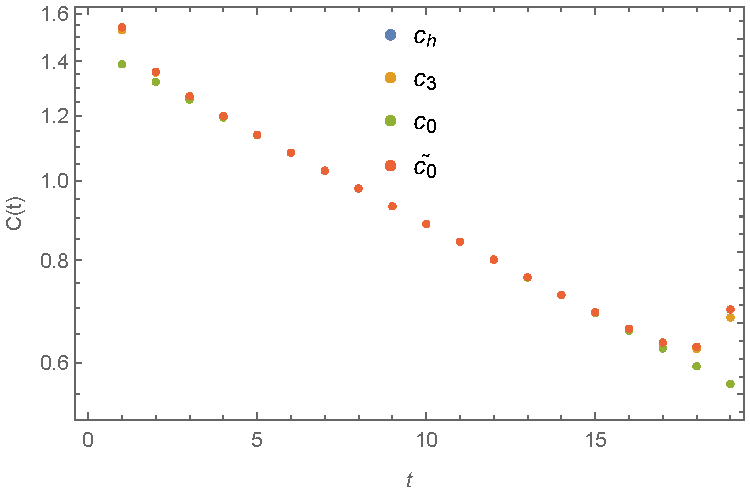
\includegraphics[width=.9\textwidth]{free-prop_real-space}
		\caption{Exact and approximate free fermion propagators at zero spatial momentum in real space, $m=\num{0.05}$. $C_h$ and $C_3$ are identical in the visualised $L_s\rightarrow\infty$ limit.}\label{fig:free_prop_real_space}
	\end{figure}

	\subsection{Influence of the Domain wall height}
	The domain wall height $M$ has a significant impact on the propagators. We refrain here from writing out the complete formula analogous to equation~\eqref{eq:exact_mom_prop_h} because of its sheer length, so (for now) we are limited to numerical observations.
	
	In figures~\ref{fig:free_prop_different_M} and~\ref{fig:free_prop_different_M_reweighted_m} we show the time dependent propagator for different domain wall heights where we $C_h$ and $C_3$ are again calculated exactly (and coincide).
	
	\begin{figure}[htp]
		\centering
		\includegraphics[width=.45\textwidth]{{free-prop_real-space_M0.25-C3}}
		\includegraphics[width=.45\textwidth]{{free-prop_real-space_M0.5-C3}}
		\caption{Exact and approximate free fermion propagators at zero spatial momentum in real space, bare mass $m=\num{0.05}$, $C_0$ and $\tilde C_0$. Domain wall heights: $M=\num{0.25}$, $M=\num{0.5}$.}\label{fig:free_prop_different_M}
	\end{figure}

	In order to approximate $C_h$, we substitute the approximate correlators
	\begin{align}
		C_0(t) &\mapsto\left(1-(1-M)^2\right) C_0(t)\label{eq:rescale_C0}
	\end{align}
	as well as the bare mass
	\begin{align}
	m &\mapsto m\left(1-(1-M)^2\right)\,.\label{eq:rescale_m}
	\end{align}
	We do not provide an analytic proof for the above formula, though hard staring at the propagator-like terms (22) in Ref.~\cite{hands_thirring2016} suggests that it looks plausible.
	With this additional modification $C_h$ and $C_3$ are well approximated by $C_0$ even for small domain wall heights $M\sim\num{0.1}$ as can be seen in figure~\ref{fig:free_prop_different_M_reweighted_m}.

	\begin{figure}[htp]
		\centering
		\includegraphics[width=.45\textwidth]{{free-prop_real-space_M0.0}}
		\includegraphics[width=.45\textwidth]{{free-prop_real-space_M0.25}}\\
		\includegraphics[width=.45\textwidth]{{free-prop_real-space_M0.5}}
		\includegraphics[width=.45\textwidth]{{free-prop_real-space_M0.75}}
		\caption{Exact and approximate free fermion propagators at zero spatial momentum in real space, bare mass $m=\num{0.05}$, $C_0$ and $\tilde C_0$ rescaled as in eq.~\eqref{eq:rescale_C0}, $m$ rescaled as in eq.~\eqref{eq:rescale_m}. Domain wall heights top: $M=0$, $M=\num{0.25}$; bottom: $M=\num{0.5}$, $M=\num{0.75}$.}\label{fig:free_prop_different_M_reweighted_m}
	\end{figure}

	Both $C_h$ and $C_3$ show rather unintuitive behaviour at the edges $t\approx 0$ and $t\approx L_t$. The deviations from the scaling at intermediate times, though always positive, appear to be smallest around $M\approx\num{0.5}$.
	
	\subsection{Influence of the Domain wall separation}
	We show the behaviour of the propagators at small domain wall separations in figure~\ref{fig:free_prop_different_Ls}. $C_h$ exhibits significant deviations from the case discussed above for $L\lesssim 6$, whereas $C_3$ remains virtually unchanged until $L\lesssim 3$. We did not search for a good approximation of the deviation (yet), though we know analytically that it has to be of order $\eto{-L_s}$ in both cases. The leading order term in $C_h$ reads
	{\fontsize{2}{2}
	\begin{align}
		\begin{split}
			-\eto{-\alpha L_s}& \left( 4 \sin ^2\left(\frac{\text{p0}}{2}\right) \left(-3 \sqrt{5-4 \cos (\text{p0})}+2 \cos (\text{p0}) \left(\sqrt{5-4 \cos (\text{p0})}+2\right)-5\right)\right.\\
			&\quad\times \left(3 m^2 \left(\sqrt{5-4 \cos (\text{p0})}+1\right)-\cos (2 \text{p0}) \left(m^2 \left(\sqrt{5-4 \cos (\text{p0})}+5\right)+3 \sqrt{5-4 \cos (\text{p0})}+13\right)+\cos (\text{p0}) \left(3 m^2+16 \sqrt{5-4 \cos (\text{p0})}+47\right)\right.\\
			&\left.\left.\qquad+m \left(m \cos (3 \text{p0})-4 i \sin (\text{p0}) \left(\cos (2 \text{p0})-2 \left(\sqrt{5-4 \cos (\text{p0})}+4\right) \cos (\text{p0})+3 \sqrt{5-4 \cos (\text{p0})}+8\right)\right)+\cos (3 \text{p0})-13 \sqrt{5-4 \cos (\text{p0})}-35\right)\right)/\\
			&\left(\left(-2 \cos (\text{p0})+\sqrt{5-4 \cos (\text{p0})}+3\right) (\cos (\text{p0})-1)\right.\\
			&\quad \left.\times \left(m^2 \sqrt{5-4 \cos (\text{p0})}-2 \cos (\text{p0}) \left(-m^2+\sqrt{5-4 \cos (\text{p0})}+3\right)-\left(m^2-1\right) \cos (2 \text{p0})+2 \sqrt{5-4 \cos (\text{p0})}+5\right)^2\right)
		\end{split}
	\end{align}}
	and the corresponding term in $C_3$ reads
	{\fontsize{2}{2}
	\begin{align}
		\begin{split}
			\eto{-\alpha L_s}& \left( 4  \sin ^2\left(\frac{p_0}{2}\right) \left(-3 \sqrt{5-4 \cos (p_0)}+2 \cos (p_0) \left(\sqrt{5-4 \cos (p_0)}+2\right)-5\right)\right.\\
			&\left.\quad\times \left(-2 i \cos (p_0) \left(2 m^2+\sqrt{5-4 \cos (p_0)}+2\right)+i \left(2 m^2 \left(\sqrt{5-4 \cos (p_0)}+3\right)+3 \sqrt{5-4 \cos (p_0)}+5\right)+2 m \sin (p_0) \left(-2 \cos (p_0)+\sqrt{5-4 \cos (p_0)}+3\right)\right)\right)/\\
			&\left(\sqrt{5-4 \cos (p_0)} \left(-2 \cos (p_0)+\sqrt{5-4 \cos (p_0)}+3\right) (\cos (p_0)-1)\right.\\
			&\quad \left.\times \left(m^2 \left(-\sqrt{5-4 \cos (p_0)}\right)+\left(m^2-1\right) \cos (2 p_0)+2 \cos (p_0) \left(-m^2+\sqrt{5-4 \cos (p_0)}+3\right)-2 \sqrt{5-4 \cos (p_0)}-5\right)\right)\,.
		\end{split}
	\end{align}}
	We find that both expressions contain first order $\eto{-\alpha L_s}$-terms but $C_3$ has only imaginary and order $\ordnung{m}$ suppressed contributions, resulting in smaller finite $L_s$ effects.
	
	\begin{figure}[htp]
		\centering
		\includegraphics[width=.45\textwidth]{{free-prop_real-space_Ls3}}
		\includegraphics[width=.45\textwidth]{{free-prop_real-space_Ls4}}\\
		\includegraphics[width=.45\textwidth]{{free-prop_real-space_Ls5}}
		\includegraphics[width=.45\textwidth]{{free-prop_real-space_Ls6}}
		\caption{Exact and approximate free fermion propagators at zero spatial momentum in real space, bare mass $m=\num{0.05}$, domain wall separations top: $L_3=3$, $L_s=4$; bottom: $L_s=5$, $L_s=6$.}\label{fig:free_prop_different_Ls}
	\end{figure}
	
	\section{Domain wall fermions with the Wilson kernel}
	Let us now have a look at the DW fermion formulation using the Wilson kernel as described in Ref.~\cite{worthy2021} (see eq.~4) instead of the Shamir kernel employed up this point. The free Dirac operator at infinite DW separation can be expressed as
	\begin{align}
		(D_0)_{ss'} &= \left(b_- + \im \slashed{\bar p}\right)\left(P_-\delta_{s+1,s'} + P_+\delta_{s-1,s'}\right) + \left(b_+ + \im \slashed{\bar p}\right)\delta_{ss'}\,,\\
		(D_0^\dagger)_{ss'} &= \left(P_-\delta_{s,s'+1} + P_+\delta_{s,s'-1}\right)\left(b_- - \im \slashed{\bar p}\right) + \left(b_+ - \im \slashed{\bar p}\right)\delta_{ss'}\,,
	\end{align}
	where we used the convention from Ref.~\cite{hands_thirring2016} (eq.~22) with minor modifications:
	\begin{align}
		P_\pm &= \frac12\left(\mathds{1}\pm\gamma_3\right)\,,\\
		\bar p_\mu &= \sin p_\mu\,,\\
		b_\pm &= \pm1-M+\sum_\mu\left(1-\cos p_\mu\right)\,.
	\end{align}

	Following the Appendix A from Ref.~\cite{hands_thirring2016}, the first step in the derivation of the free fermion propagator is to calculate the matrix product
	\begin{align}
		\begin{split}
			(D_0D_0^\dagger)_{ss'} &= \left(b_+^2+{\bar p}^2\right)\delta_{ss'}
			+ \left(\left(b_+ + \im \slashed{\bar p}\right)\delta_{ss''} \left(P_-\delta_{s'',s'+1} + P_+\delta_{s'',s'-1}\right)\left(b_- - \im \slashed{\bar p}\right) + h.c.\right)\\
			&\quad + \left(b_-^2+\im b_-\slashed{\bar p}\right)\left(P_-\delta_{ss'}+P_+\delta_{ss'}\right) + \left(-\im b_-\slashed{\bar p}+{\bar p}^2\right)\left(P_-\delta_{ss'}+P_+\delta_{ss'}\right)
		\end{split}\\
		\begin{split}
			&= \left(b_+^2+{\bar p}^2\right)\delta_{ss'}
			+ \left(\left(b_+b_- + \im b_- \slashed{\bar p}\right)\left(P_-\delta_{s,s'+1} + P_+\delta_{s,s'-1}\right)\right.\\
			&\qquad \left.+ \left(- \im b_+ \slashed{\bar p} + {\bar p}^2\right)\left(P_+\delta_{s,s'+1} + P_-\delta_{s,s'-1}\right) + h.c.\right)\\
			&\quad + \left(b_-^2+{\bar p}^2\right)\delta_{ss'}
		\end{split}\\
		&= \left(b_+^2+b_-^2+2\bar p^2\right)\delta_{ss'} + \left(b_+b_- + {\bar p}^2\right)\left(\delta_{s,s'+1} + \delta_{s,s'-1}\right)\,.
	\end{align}

	We postpone the further derivation of the full propagator for now and focus on the most important case when $M=1$ and $p=(p_0,0,0)$ simplifying
	\begin{align}
		b_+b_- + {\bar p}^2 &= (1-\cos p_0)(-1-\cos p_0) + \sin^2 p_0\\
		&= \cos^2 p_0 - 1 + \sin^2 p_0\\
		&= 0
	\end{align}
	and
	\begin{align}
		b_+^2+b_-^2+2\bar p^2 &= (1-\cos p_0)^2 + (-1-\cos p_0)^2 + 2\sin^2 p_0\\
		&= 2 + 2\cos^2 p_0 + 2\sin^2 p_0\\
		&= 4\,,
	\end{align}
	thus
	\begin{align}
		D_0D_0^\dagger = 4 \mathds{1}\,.
	\end{align}

	This result is totally unphysical since the Greens function $D_0^{-1}=D_0^\dagger(D_0D_0^\dagger)^{-1}$ and therefore the propagator does not have any poles because of the trivial denominator. No particles are described in this way.
	
	\clearpage
	\printbibliography
\end{document}
.